\section{Klasy złożoności obliczeniowej}

Niech $M$ będzie maszyną Turinga. \vocab{Złożoność czasowa} $M$ to funkcja $f\colon \NN \to \NN$, gdzie $f(n)$ to maksymalna liczba kroków, jakie $M$ wykonuje na wejściu długości $n$. \vocab{Złożoność pamięciowa} $M$ to funkcja $g\colon \NN \to \NN$, gdzie $g(n)$ to maksymalna liczba komórek taśmy, jakie $M$ używa na wejściu długości $n$. Definiujemy klasy języków:
\[ \TIME(t(n)) = \left\{ L \mid \exists M \text{ rozstrzygająca o } L \text{ w czasie } \sO(t(n)) \right\} \]
oraz
\[ \SPACE(s(n)) = \left\{ L \mid \exists M \text{ rozstrzygająca o } L \text{ w pamięci } \sO(s(n)) \right\}. \]

Korzystając z tych definicji, możemy również zdefiniować klasę języków decyzyjnych, które są rozstrzygalne w czasie wielomianowym
\[ \Pclass = \bigcup_{k = 1}^\infty \TIME\left(n^k\right), \]
klasę języków decyzyjnych, które są rozstrzygalne w czasie wykładniczym
\[ \EXPclass = \bigcup_{k = 1}^\infty \TIME\left(2^{n^k}\right) \]
oraz klasy języków, które są rozstrzygalne w pamięci wielomianowej i wykładniczej, odpowiednio
\[ \PSPACEclass = \bigcup_{k = 1}^\infty \SPACE\left(n^k\right), \]
\[ \EXPSPACEclass = \bigcup_{k = 1}^\infty \SPACE\left(2^{n^k}\right). \]

Oczywistym jest, że $\Pclass \subseteq \EXPclass$ i $\PSPACEclass \subseteq \EXPSPACEclass$. Łatwo zauważyć również, że $\Pclass \subseteq \PSPACEclass$ i $\EXPclass \subseteq \EXPSPACEclass$ (konsumowanie pamięci zajmuje czas). Możemy natomiast udowodnić nieco mniej oczywisty fakt.
\begin{fact}
    Zachodzi inkluzja $\PSPACEclass \subseteq \EXPclass$.
\end{fact}
\begin{proof}
    Maszyna Turinga ma wykładniczo wiele konfiguracji taśmy w stosunku do długości tej taśmy. Nie istnieje więc problem, który można rozwiązać w pamięci wielomianowej, ale nie można go rozwiązać w czasie wykładniczym.
\end{proof}

\subsection{Niedeterministyczna maszyna Turinga}

Niedeterministyczna maszyna Turinga to uogólnienie maszyny Turinga, które pozwala na wiele możliwych stanów, w których może znaleźć się maszyna w danym momencie.

\begin{definition}
    Niedeterministyczna maszyna Turinga to krotka
    \[ M = (Q, \Sigma, \Gamma, \delta, q_0, q_Y, q_N, \blank),\]
    gdzie
    \begin{itemize}[noitemsep]
        \item $Q$ to skończony zbiór stanów,
        \item $\Sigma$ to skończony alfabet wejściowy,
        \item $\Gamma$ to skończony alfabet taśmy, taki że $\Sigma \subset \Gamma$ oraz $\blank \in \Gamma \setminus \Sigma$,
        \item $\delta \subseteq \left(Q \times \Gamma\right) \times \left(Q \times \Gamma \times \{\hookleftarrow , \hookrightarrow\}\right)$ to \textbf{relacja}  przejścia,
        \item $q_0 \in Q$ to stan początkowy,
        \item $q_Y \in Q$ to stan akceptujący,
        \item $q_N \in Q$ to stan odrzucający.
    \end{itemize}

    \vocab{Ścieżką obliczeń} nazwiemy skończony ciąg stanów i symboli taśmy, który zaczyna się w stanie $q_0$ i jest osiągalny za pomocą relacji przejścia $\delta$.

    Niedeterministyczna maszyna Turinga akceptuje słowo $x$ o długości $n$, jeśli istnieje ścieżka obliczeń, która kończy się w stanie $q_Y$. Język jest rozstrzygany przez niedeterministyczną maszynę Turinga $M$ w czasie $f(n)$, jeśli dla każdego słowa $x$ o długości $n$ każda ścieżka obliczeń kończy się w czasie $f(n)$ oraz $M$ akceptuje $x$ wtedy i tylko wtedy, gdy $x \in L$.
\end{definition}

Analogicznie do już zdefiniowanych klas złożoności obliczeniowej, definiujemy klasy języków decyzyjnych, które są rozstrzygalne przez niedeterministyczną maszynę Turinga; oznaczamy je jako $\NPclass$, $\NPSPACEclass$, $\NEXPclass$ i tym podobne.

\subsection{Redukcje wielomianowe, jeszcze raz o trudności i zupełności}

\begin{definition}[redukcja wielomianowa \textit{many-one}]\label{d:poly reduction}
    Język $A$ \vocab{redukuje się} do języka $B$ w czasie wielomianowym, co zapisujemy jako $A \leq_m^p B$, jeśli istnieje funkcja $f$ obliczalna w czasie wielomianowym taka, że dla każdego $x \in \Sigma^*$ zachodzi
    \[ x \in A \iff f(x) \in B. \]
\end{definition}

Nasze definicje trudności i zupełności języków w klasach $\REclass$, $\coREclass$ czy też szerszych $\Sigma_i$ i $\Pi_i$ nie mają zbyt dużego sensu w kontekście klas $\Pclass$, $\NPclass$, $\PSPACEclass$ czy $\NEXPclass$ (z powodu twierdzenia \ref{t:nontrivial R language is R-complete}). W tych klasach zamiast zwykłej redukcji funkcją obliczalną używamy redukcji wielomianowej, co odpowiednio zmienia definicje trudności i zupełności.

\subsection{Problem SAT}

Problem SAT (\textit{satisfiability}) to problem spełnialności danej formuły logicznej, a więc stwierdzenia, czy istnieje takie wartościowania jej zmiennych, które sprawia, że formuła jest prawdziwa.

Często używana jest wersja problemu SAT, w której formuła jest w koniunkcyjnej postaci normalnej (CNF, \textit{conjunctional normal form}), a więc jest koniunkcją klauzul, gdzie klauzula to alternatywa literałów, a literał to zmienna lub jej negacja. Przykładowo, formuła
\[ (x_1 \lor \neg x_2) \land (\neg x_1 \lor x_2 \lor x_3 \lor x_4) \]
jest w postaci CNF.

\begin{fact}[algorytm Tseitina]
    Każdą formułę logiczną można sprowadzić do postaci CNF w czasie wielomianowym, a rozmiar formuły wyjściowej będzie liniowy w stosunku do rozmiaru formuły wejściowej.
\end{fact}

\begin{theorem}[Cooka-Levina]\label{t:Cook-Levin}
    Problem SAT jest $\NPclass$-zupełny.
\end{theorem}
\begin{proof}
    Łatwo zaobserwować, że problem SAT jest w klasie $\NPclass$. Niedeterministyczna maszyna Turinga może niedeterministycznie wybrać wartościowanie zmiennych i sprawdzać, czy formuła jest spełniona. Pokażemy, że problem SAT jest $\NPclass$-trudny, a więc jest $\NPclass$-zupełny.

    Niech $H$ będzie problemem takim, że
    \[ H = \left\{\encode{N, x, 0^t} \Bigm| \parbox{15em}{\footnotesize niedeterministyczna maszyna Turinga $N$ akceptuje słowo $x$ w $t$ krokach}\right\}. \]
    Łatwo zauważyć, że $H$ jest problemem $\NPclass$-trudnym (można do niego sprowadzić każdy inny problem z $\NPclass$) oraz sam należy do $\NPclass$ (maszyna $M_H$ może niedeterministycznie wybierać relację $\delta$ i symulować działanie maszyny $N$).
    Wystarczy więc pokazać, że $H$ redukuje się do SAT.

    Zdefiniujemy następujące zmienne logiczne:
    \begin{itemize}
        \item $Q_{i, k}$: w $i$-tym kroku maszyna $M_H$ jest w stanie $q_k$,
        \item $P_{i, j}$: w $i$-tym kroku głowica maszyny $M_H$ jest na $j$-tym polu,
        \item $S_{i, j, l}$: w $i$-tym kroku na $j$-tym polu taśmy znajduje się symbol $l$.
    \end{itemize}
    Będziemy chcieli tak skonstruować formułę logiczną $\phi$, że $\phi$ jest spełnialna wtedy i tylko wtedy, gdy istnieje ścieżka obliczeń maszyny $M_H$ akceptująca słowo $x$ czasie wielomianowym. W tym celu do formuły $\phi$ dodajemy klauzule, które:
    \begin{enumerate}
        \item wymuszają, że w każdym kroku maszyna $M_L$ znajduje się w dokładnie jednym stanie, to jest
        \[ \bigwedge_i \left(Q_{i, 1} \lor \cdots \lor Q_{i, |Q|}\right), \]
        \[ \bigwedge_i \bigwedge_{k \neq k'} \left(\neg Q_{i, k} \lor \neg Q_{i, k'}\right); \]
        \item wymuszają, że w każdym kroku głowica maszyny $M_L$ znajduje się na dokładnie jednym polu;
        \item wymuszają, że w każdym kroku na każdym polu taśmy znajduje się dokładnie jeden symbol;
        \item wymuszają zgodność słowa wejściowego, to jest
        \[ \bigwedge_{j \leq |x|} \left(S_{1, j, x_j}\right) \quad \bigwedge_{|x| < j} \left(S_{1, j, \blank}\right); \]
        \item wymaszają poprawność przejść między stanami;
        \item wymuszają, że istnieje ścieżka obliczeń, która kończy się w stanie akceptującym, to jest
        \[ \left( Q_{1, Y} \lor Q_{2, Y} \lor \cdots \right). \]
    \end{enumerate}
    Klauzul tych jest wielomianowo wiele, więc pokazaliśmy, że $H \leq_m^p \textsc{SAT}$, a więc problem SAT jest $\NPclass$-zupełny.
\end{proof}

\section{Klasyczne problemy $\NPclass$-zupełne}

Dowodząc $\NPclass$-zupełności problemu, wystarczy pokazać, że problem jest w klasie $\NPclass$ oraz że jest $\NPclass$-trudny. Tę pierwszą cześć z reguły będziemy zostawiać jako ćwiczenie dla Czytelnika, gdyż jest to zwykle dosyć proste --- niedeterministyczna maszyna Turinga może po prostu wybierać odpowiedź (wartościowanie formuły logicznej, podzbiór wierzchołków w grafie, itp.) i sprawdzać, czy jest dobrym \vocab{świadkiem}, czyli czy spełnia warunki problemu.

\subsection{Problem 3-SAT i jego bardziej szczegółowe wersje}

Problem spełnialności formuł w postaci CNF, gdzie każda klauzula ma co najwyżej $k$ literałów będziemy nazywać problemem $k$-SAT. Problem 3-SAT jest $\NPclass$-zupełny, co udowodnimy jako twierdzenie \ref{t:3-SAT}, jednak już 2-SAT jest w klasie $\Pclass$, a rozwiązujący go algorytm jest opisany chociażby na \href{https://cp-algorithms.com/graph/2SAT.html}{cp-algorithms}.

Możemy również w inny sposób wprowadzić ograniczenia na formułę, które nie sprawią, że problem przestanie być $\NPclass$-zupełny, a może stać się bardziej przydatny.
Takim ograniczeniem będzie chociażby maksymalna liczby wystąpień każdej zmiennej w formule. Problem $k$-SAT, w którym każda zmienna występuje co najwyżej $\ell$ razy nazywamy $(k, \ell)$-SAT. W ramach twierdzenia \ref{t:3,3-SAT} pokażemy, że problem $(3, 3)$-SAT również jest $\NPclass$-zupełny.

\begin{remark}
    Czesto można spotkać również alternatywną definicję problemu $k$-SAT; mianowicie, że jest to problem spełnialności formuł w postaci CNF, gdzie każda klauzula ma \emph{dokładnie} $k$ literałów.

    Zazwyczaj nie ma to żadnego znaczenia w kontekście przeprowadzanych redukcji, ale jeśli zdefiniujemy $(3, 3)$-SAT jako problem spełnialności formuł w postaci CNF, gdzie każda klauzula ma \emph{dokładnie} trzy literały, a każda zmienna występuje co najwyżej trzy razy, to ten problem jest już w $\Pclass$, a nawet więcej --- formuła w takiej postaci zawsze jest tautologią, co dociekliwy Czytelnik może udowodnić za pomocą twierdzenia Halla o kojarzeniu małżeństw.
\end{remark}

Warto zauważyć, że problem SAT, w którym każda zmienna występuje co najwyżej dwa razy jest w $\Pclass$, podobnie jak problem SAT, w którym każda klauzula ma co najwyżej jeden niezanegowany literał. Oba te fakty dociekliwy Czytelnik powinien udowodnić.

\begin{theorem}\label{t:3-SAT}
    Problem 3-SAT jest $\NPclass$-zupełny.
\end{theorem}
\begin{proof}
    Zauważmy, że klauzula
    \[ a_1 \lor a_2 \lor \cdots \lor a_n \]
    jest równoważna formule
    \[ ((a_1 \lor a_2) \Leftrightarrow b) \land (b \lor a_3 \lor \cdots \lor a_n), \]
    a z kolei
    \[ ((a_1 \lor a_2) \Leftrightarrow b) \]
    jest równoważne
    \[ (\neg a_1 \lor b) \land (\neg a_2 \lor b) \land (a_1 \lor a_2 \lor \neg b). \]
    W ten sposób możemy zredukować rozmiar każdej klauzuli z $n$ do $\max(3, n-1)$. Powtarzając ten proces wielokrotnie, dokonujemy redukcji problemu SAT do 3-SAT.
\end{proof}

\begin{theorem}\label{t:3,3-SAT}
    Problem $(3, 3)$-SAT jest $\NPclass$-zupełny.
\end{theorem}
\begin{proof}
    Jeśli jakaś zmienna $x$ występuje $m > 3$ razy w formule $\phi$, to jej $i$-te wystąpienie możemy zastąpić nową zmienną $x_i$, a do formuły $\phi$ dodać klauzule
    \[ (x_1 \lor \ol{x_2}) \land (x_2 \lor \ol{x_3}) \land \ldots \land (x_{m-1} \lor \ol{x_m}) \land (x_m \lor \ol{x_1}). \]
    Jeśli $x_1$ jest fałszywe, to fałszywe musi być również $x_2$, a tym samym $x_3, \ldots, x_m$, co oznacza, że wszystkie zmienne $x_i$ muszą być albo fałszywe, albo prawdziwe. W ten sposób zredukowaliśmy $m$-krotne występowanie zmiennej $x$ do 3-krotnego występowania zmiennych $x_i$, a więc 3-SAT $\leq_m^p$ $(3, 3)$-SAT.
\end{proof}

\subsection{Problem \textsc{Independent Set}}

Problem \textsc{Independent Set} to problem stwierdzenia, czy w danym grafie nieskierowanym $G$ istnieje zbiór $k$ wierzchołków niezależnych, czyli takich, że żadne dwa z nich nie są połączone krawędzią.

\begin{theorem}
    Problem \textsc{Independent Set} jest $\NPclass$-zupełny.
\end{theorem}
\begin{proof}
    Przeprowadzimy redukcję problemu 3-SAT do problemu \textsc{Independent Set}. Niech $\phi$ będzie formułą w postaci CNF, gdzie każda klauzula ma co najwyżej trzy literały. Zbudujemy graf $G$ w następujący sposób:
    \begin{itemize}
        \item Dla każdego literału w każdej klauzuli tworzymy wierzchołek; łączymy krawędziamy wierzchołki odpowiadające literałom w tej samej klauzuli.
        \item Łączymy krawędziami wierzchołki odpowiadające przeciwstawnym literałom w różnych klauzulach (to znaczy takie, że jeden jest zanegowany, a drugi nie).
    \end{itemize}
    Graf $G$ ma wtedy zbiór $k$ wierzchołków niezależnych wtedy i tylko wtedy, gdy formuła $\phi$ zawierająca $k$ klauzul jest spełnialna. Zbiór $k$ wierzchołków niezależnych w grafie $G$ odpowiada zbiorowi $k$ wartościowań zmiennych, które spełniają formułę $\phi$.

    W ten sposób pokazaliśmy, że 3-SAT $\leq_m^p$ \textsc{Independent Set}, a więc problem \textsc{Independent Set} jest $\NPclass$-trudny. Jest on również w $\NPclass$, więc jest $\NPclass$-zupełny.
\end{proof}

\begin{figure}[H]
    \centering
    \SetCoordinates[xAngle=-30,yLength=1.2,xLength=1]
    \SetLayerDistance{-2.5}
    \begin{tikzpicture}[multilayer=3d,scale=0.8]
        \Vertex[x=1,y=2,label=$x$,layer=1,color=AccColor3]{x_1}
        \Vertex[x=3,y=2,label=$y$,layer=1,color=AccColor2]{y_1}
        \Vertex[x=2,y=0,label=$z$,layer=1,color=AccColor2]{z_1}
        \Edge(x_1)(y_1)
        \Edge(x_1)(z_1)
        \Edge(y_1)(z_1)

        \Vertex[x=1,y=2,label=$\ol{x}$,layer=2,color=AccColor2]{x_2}
        \Vertex[x=3,y=2,label=$\ol{y}$,layer=2,color=AccColor2]{y_2}
        \Vertex[x=2,y=0,label=$z$,layer=2,color=AccColor3]{z_2}
        \Edge(x_2)(y_2)
        \Edge(x_2)(z_2)
        \Edge(y_2)(z_2)

        \Vertex[x=1,y=2,label=$\ol{x}$,layer=3,color=AccColor2]{x_3}
        \Vertex[x=3,y=2,label=$y$,layer=3,color=AccColor3]{y_3}
        \Vertex[x=2,y=0,label=$\ol{z}$,layer=3,color=AccColor2]{z_3}
        \Edge(x_3)(y_3)
        \Edge(x_3)(z_3)
        \Edge(y_3)(z_3)

        \Edge[style=dashed](x_1)(x_2)
        \Edge[style=dashed](y_1)(y_2)

        \Edge[style=dashed](y_2)(y_3)
        \Edge[style=dashed](z_2)(z_3)

        \Edge[style=dashed,bend=15](x_1)(x_3)
        \Edge[style=dashed,bend=-15](z_1)(z_3)
    \end{tikzpicture}

    \caption{Graf odpowiadający formule $\phi = (x \lor y \lor z) \land (\neg x \lor \neg y \lor z) \land (\neg x \lor y \lor \neg z)$. Istnieje zbiór $k = 3$ wierzchołków niezależnych (zaznaczony), a więc formuła $\phi$ jest spełnialna.}
\end{figure}

\subsection{Problem \textsc{Clique}}

Problem \textsc{Clique} to problem stwierdzenia, czy w danym grafie nieskierowanym $G$ istnieje klika (podgraf pełny) rzędu $k$.

\begin{theorem}
    Problem \textsc{Clique} jest $\NPclass$-zupełny.
\end{theorem}
\begin{proof}
    Zamiast rozwiązywać problem \textsc{Clique} na grafie $G$, można rozwiązać problem \textsc{Independent Set} na dopełnieniu grafu (czyli takim grafie $\ol{G}$, w którym dwa wierzchołki są połączone krawędzią wtedy i tylko wtedy, gdy nie są połączone w grafie $G$). Wtedy zbiór $k$ wierzchołków niezależnych w grafie $\overline{G}$ odpowiada zbiorowi $k$ wierzchołków tworzących klikę w grafie $G$. Te dwa problemy są więc równoważne.
\end{proof}

\subsection{Problem 3-\textsc{Color}}

Problem 3-\textsc{Color} to problem stwierdzenia, czy dany graf nieskierowany $G$ można pokolorować trzema kolorami w taki sposób, żeby żadne dwa sąsiednie wierzchołki nie miały tego samego koloru.

\begin{theorem}
    Problem 3-\textsc{Color} jest $\NPclass$-zupełny.
\end{theorem}
\begin{proof}
    Przeprowadzimy redukcję problemu 3-SAT do problemu 3-\textsc{Color}. Niech $\phi$ będzie formułą w postaci CNF, gdzie każda klauzula ma co najwyżej trzy literały. Zbudujemy graf $G$ w taki sposób, że jego wierzchołkami będą literały (w postaci zarówno zmiennych, jak i ich negacji) oraz klauzule.
    Ponadto, do grafu $G$ dodamy specjalne wierzchołki $T$ (prawda), $F$ (fałsz) i $S$ (inny) oraz krawędzie między nimi. Dodamy również wszystkie krawędzie między wierzchołkami reprezentującymi literały a wierzchołkiem $S$ (literały powinny mieć kolor taki jak $P$ lub $F$) oraz między wierzchołkami reprezentującymi klauzule a wierzchołkami $F$ i $S$ (klauzule powinny mieć taki kolor jak $P$).

    Dla każdej klauzuli $C_i = (x \lor y \lor z)$ tworzymy dodatkowo następującą strukturę:
    \begin{figure}[H]
        \centering
        \begin{tikzpicture}[scale=0.7]
            \Vertex[x=0,y=4,label=$x$,color=AccColor2]{x}
            \Vertex[x=0,y=2,label=$y$,color=AccColor2]{y}
            \Vertex[x=0,y=0,label=$z$,color=AccColor2]{z}
            \Vertex[x=2,y=4]{a}
            \Vertex[x=2,y=2]{b}
            \Vertex[x=4,y=3]{c}
            \Vertex[x=6,y=3]{d}
            \Vertex[x=6,y=0]{e}
            \Vertex[x=8,y=1.5,label=$C_i$,color=AccColor1]{C}

            \Edge(x)(a)
            \Edge(y)(b)
            \Edge(z)(e)
            \Edge(a)(b)
            \Edge(a)(c)
            \Edge(b)(c)
            \Edge(c)(d)
            \Edge(d)(e)
            \Edge(d)(C)
            \Edge(e)(C)
        \end{tikzpicture}
    \end{figure}

    Oczywiście jeśli klauzula ma mniej niż $3$ literały, to odpowienio tę strukturę upraszczamy.
    Nietrudno zauważyć, że tak stworzony graf $G$ jest 3-kolorowalny wtedy i tylko wtedy, gdy formuła $\phi$ jest spełnialna, ponieważ nasza struktura symuluje alternatywę logiczną.

    W ten sposób pokazaliśmy, że 3-SAT $\leq_m^p$ 3-\textsc{Color}, a więc problem 3-\textsc{Color} jest $\NPclass$-trudny. Jest on również w $\NPclass$, więc jest $\NPclass$-zupełny.
\end{proof}

\subsection{Problem \textsc{(Directed) Hamiltonian Path / Cycle}}

Problem \textsc{Directed Hamiltonian Path} to problem stwierdzenia, czy w danym grafie skierowanym $G$ istnieje ścieżka Hamiltona $s \rightsquigarrow t$, czyli taka, która przechodzi przez każdy wierzchołek dokładnie raz. Problem \textsc{Hamiltonian Path} jest analogiczny, jedynie graf $G$ jest nieskierowany.

\begin{theorem}
    Problem \textsc{Directed Hamiltonian Path} jest $\NPclass$-zupełny.
\end{theorem}
\begin{proof}
    Przeprowadzimy redukcję problemu 3-SAT do problemu \textsc{Directed Hamiltonian Path}. Niech $\phi = C_1 \land \cdots \land C_k$ będzie formułą w postaci CNF, gdzie każda klauzula $C_i$ ma co najwyżej trzy literały. Zbudujemy graf skierowany $G$ w następujący sposób:
    \begin{enumerate}
        \item W grafie tworzymy dwa wyróżnione wierzchołki: $s$ oraz $t$. Dla każdej zmiennej $x_j$ tworzymy również dwa wierzchołki: $x_j$ i $\ol{x_j}$. Dodajemy krawędzie $s\,x_1$, $s\,\ol{x_1}$, $x_n\,t$, $\ol{x_n}\,t$ oraz dla każdego $1 < j < n$ krawędzie $x_j\,x_{j+1}$, $x_j\,\ol{x_{j+1}}$, $\ol{x_j}\,x_{j+1}$ i $\ol{x_j}\,\ol{x_{j+1}}$, otrzymując w ten sposób poniższy graf.
        \begin{figure}[H]
            \centering
            \begin{tikzpicture}[scale=0.6]
                \Vertex[x=0,y=0,label=$s$]{s}
                \Vertex[x=-4,y=-2,label=$x_1$,color=AccColor2]{x_1^T}
                \Vertex[x=4,y=-2,label=$\ol{x_1}$,color=AccColor2]{x_1^F}
                \Vertex[x=-4,y=-4,label=$x_2$,color=AccColor2]{x_2^T}
                \Vertex[x=4,y=-4,label=$\ol{x_2}$,color=AccColor2]{x_2^F}
                \Vertex[x=-4,y=-6,label=$x_3$,color=AccColor2]{x_3^T}
                \Vertex[x=4,y=-6,label=$\ol{x_3}$,color=AccColor2]{x_3^F}
                \Text[x=0,y=-7.5,fontsize=\Large]{$\cdots$}
                \Vertex[x=-4,y=-9,label=$x_n$,color=AccColor2]{x_n^T}
                \Vertex[x=4,y=-9,label=$\ol{x_n}$,color=AccColor2]{x_n^F}
                \Vertex[x=0,y=-11,label=$t$]{t}

                \Edge[Direct](s)(x_1^T)
                \Edge[Direct](s)(x_1^F)
                \Edge[Direct](x_1^T)(x_2^T)
                \Edge[Direct](x_1^T)(x_2^F)
                \Edge[Direct](x_1^F)(x_2^T)
                \Edge[Direct](x_1^F)(x_2^F)
                \Edge[Direct](x_2^T)(x_3^T)
                \Edge[Direct](x_2^T)(x_3^F)
                \Edge[Direct](x_2^F)(x_3^T)
                \Edge[Direct](x_2^F)(x_3^F)
                \Edge[Direct](x_n^T)(t)
                \Edge[Direct](x_n^F)(t)
            \end{tikzpicture}
        \end{figure}

        W takim grafie na pewno nie ma ścieżki Hamiltona, ponieważ musimy odwiedzić wszystkie wierzchołki, a póki co możemy odwiedzić tylko jeden z każdej pary $x_j, \ol{x_j}$.

        \item Dla każdej pary $x_j$, $\ol{x_j}$ tworzymy dodatkowe wierzchołki $a_{j, 1}, a_{j, 1}', \ldots, a_{j, k}, a_{j, k}'$ i łączymy je w następujący sposób:
        \begin{figure}[H]
            \centering
            \begin{tikzpicture}[scale=0.6]
                \Vertex[x=-7,y=-2,label=$x_j$,color=AccColor2]{x^T}
                \Vertex[x=7,y=-2,label=$\ol{x_j}$,color=AccColor2]{x^F}
                \Vertex[x=-5,y=-2,label=$a_{j, 1}$]{a_1}
                \Vertex[x=-3,y=-2,label=$a_{j, 1}'$]{a_1'}
                \Vertex[x=-1,y=-2,label=$a_{j, 2}$]{a_2}
                \Text[x=1,y=-2,fontsize=\Large]{$\cdots$}
                \Vertex[x=3,y=-2,label=$a_{j, k}$]{a_k}
                \Vertex[x=5,y=-2,label=$a_{j, k}'$]{a_k'}

                \Edge[Direct,bend=30](x^T)(a_1)
                \Edge[Direct,bend=30](a_1)(x^T)
                \Edge[Direct,bend=30](a_1)(a_1')
                \Edge[Direct,bend=30](a_1')(a_1)
                \Edge[Direct,bend=30](a_1')(a_2)
                \Edge[Direct,bend=30](a_2)(a_1')
                \Edge[Direct,bend=30](a_k)(a_k')
                \Edge[Direct,bend=30](a_k')(a_k)
                \Edge[Direct,bend=30](a_k')(x^F)
                \Edge[Direct,bend=30](x^F)(a_k')
            \end{tikzpicture}
        \end{figure}

        Teraz możemy już znaleźć ścieżkę Hamiltona; każda taka ścieżka będzie odpowiadała pewnemu wartościowaniu formuły $\phi$ (przejście ścieżką $x_j \rightsquigarrow \ol{x_j}$ oznacza wartościowanie $x_j = \text{prawda}$, a przejście ścieżką $\ol{x_j} \rightsquigarrow x_j$ oznacza wartościowanie $x_j = \text{fałsz}$).

        \item Dla każdej klauzuli $C_i$ tworzymy odpowiadający jej wierzchołek $C_i$. Jeśli klauzula $C_i$ zawiera $x_j$, to tworzymy krawędzie $a_{j, i}\,C_i$ oraz $C_i\,a_{j, i}'$, a jeśli zawiera $\ol{x_j}$, to tworzymy krawędzie $C_i\,a_{j, i}$ oraz $a_{j, i}'\,C_i$. Na przykład dla klauzuli $C_1$ zawierającej $x_j$ otrzymujemy graf
        \begin{figure}[H]
            \centering
            \begin{tikzpicture}[scale=0.6]
                \Vertex[x=-7,y=-2,label=$x_j$,color=AccColor2]{x^T}
                \Vertex[x=-5,y=-2,label=$a_{j, 1}$]{a_1}
                \Vertex[x=-3,y=-2,label=$a_{j, 1}'$]{a_1'}
                \Vertex[x=-1,y=-2,label=$a_{j, 2}$]{a_2}
                \Vertex[x=1,y=0.5,label=$C_1$,color=AccColor1]{C_1}

                \Edge[Direct,bend=30](x^T)(a_1)
                \Edge[Direct,bend=30](a_1)(x^T)
                \Edge[Direct,bend=30](a_1)(a_1')
                \Edge[Direct,bend=30](a_1')(a_1)
                \Edge[Direct,bend=30](a_1')(a_2)
                \Edge[Direct,bend=30](a_2)(a_1')
                \Edge[Direct,bend=30](a_1)(C_1)
                \Edge[Direct,bend=-20](C_1)(a_1')
            \end{tikzpicture}
        \end{figure}
    \end{enumerate}

    Nietrudno zauważyć, że w grafie $G$ istnieje scieżka Hamiltona $s \rightsquigarrow t$ (przechodząca również przez wierzchołki $C_i$) wtedy i tylko wtedy, gdy formuła $\phi$ jest spełnialna. W ten sposób pokazaliśmy, że 3-SAT $\leq_m^p$ \textsc{Directed Hamiltonian Path}, a więc problem \textsc{Directed Hamiltonian Path} jest $\NPclass$-trudny. Jest on również w $\NPclass$, więc jest $\NPclass$-zupełny.
\end{proof}

\begin{theorem}
    Problem \textsc{Hamiltonian Path} jest $\NPclass$-zupełny.
\end{theorem}
\begin{proof}
    Pokażemy redukcję problemu \textsc{Directed Hamiltonian Path} do \textsc{Hamiltonian Path}. Niech $G$ będzie grafem skierowanym, a $G'$ grafem nieskierowanym, który otrzymujemy z $G$ w taki sposób, że każdy wierzchołek $v \in G$ przepisujemy do $G'$ jako trzy (połączone ścieżką) wierzchołki: $v_\text{in}$, $v_\text{mid}$ i $v_\text{out}$, a każdą krawędź skierowaną $uv \in G$ przepisujemy do grafu $G'$ jako krawędź $u_\text{out}v_\text{in}$.

    Oczywiście nie każda nieskierowana ścieżka w grafie $G'$ odpowiada dokładnie jednej skierowanej ścieżce w grafie $G$, ale jeśli ograniczymy się tylko do ścieżek Hamiltona, to ten fakt istotnie zachodzi, ponieważ taka ścieżka musi przechodzić dokładnie raz przez wszystkie wierzchołki $v_\text{mid}$ (a więc raz wchodzi i raz wychodzi z wierzchołka).
    W ten sposób pokazaliśmy, że \textsc{Directed Hamiltonian Path} $\leq_m^p$ \textsc{Hamiltonian Path}, a więc problem \textsc{Hamiltonian Path} jest $\NPclass$-trudny. Jest on również w $\NPclass$, więc jest $\NPclass$-zupełny.
\end{proof}

Bardzo łatwo zauważyć, że problemy \textsc{Directed Hamiltonian Cycle} i \textsc{Hamiltonian Cycle} również są $\NPclass$-zupełne --- w dowodach wystarczy dodać krawędź $ts$.

\subsection{Problemy \textsc{Set Cover} i X3C}

Problem \textsc{Set Cover} to problem stwierdzenia, czy dany zbiór $B = \{b_1, \ldots, b_n\}$ można reprezentować jako sumę mnogościową co najwyżej $t$ zbiorów z danej rodziny podzbiorów $B$, oznaczanej jako $\sS = \{S_1, \ldots, S_m\} \subseteq \sP(B)$.
Taka reprezentacja nazywa się \vocab{pokryciem} zbioru.

Podobnie jak dla problemu SAT, będziemy chcieli wprowadzić pewne ograniczenie danych tego problemu, które, jak udowodnimy, będzie równoważne pełnemu problemowi. W tym przypadku będzie to problem X3C (\textit{exact cover by 3-sets}), w którym dodatkowo $n = 3t$ oraz $|S_i| = 3$ dla każdego $i$ (z czego wynika, że zbiory z $\sS$ muszą być rozłączne).

\begin{theorem}\label{t:Set Cover}
    Problem \textsc{Set Cover} jest $\NPclass$-zupełny.
\end{theorem}
\begin{proof}
    Pokażemy redukcję problemu 3-SAT do problemu \textsc{Set Cover}. Niech $\phi = C_1 \land \cdots \land C_k$ będzie formułą w postaci CNF, gdzie każda klauzula $C_i$ ma co najwyżej trzy literały. Niech zbiór $B$ zawiera zmienne oraz klauzule:
    \[ B = \{x_1, \ldots, x_n, C_1, \ldots, C_k\}, \]
    a każda zmienna $x_j$ ma dwa odpowiadające zbiory:
    \begin{align*}
        S_{x_j = 0} &= \{x_j\} \cup \left\{C_i \Bigm| \text{\footnotesize klauzula $C_i$ zawiera (zaprzeczony) literał $\ol{x_j}$}\right\}, \\
        S_{x_j = 1} &= \{x_j\} \cup \left\{C_i \Bigm| \text{\footnotesize klauzula $C_i$ zawiera (niezaprzeczony) literał $x_j$}\right\},
    \end{align*}
    należące do rodziny $\sS$.

    Zbiór $B$ można pokryć $n$ zbiorami z $\sS$ wtedy i tylko wtedy, gdy formuła $\phi$ jest spełnialna (jeśli formuła nie jest spełnialna, to nie uda się pokryć wszystkich klauzul $C_i$, a w przeciwnym wypadku będziemy mogli to zrobić wybierając jeden z każdej pary zbiorów $S_{x_j = b}$). W ten sposób pokazaliśmy, że 3-SAT $\leq_m^p$ \textsc{Set Cover}, a więc problem \textsc{Set Cover} jest $\NPclass$-trudny. Jest on również w $\NPclass$, więc jest $\NPclass$-zupełny.
\end{proof}

\begin{theorem}
    Problem X3C jest $\NPclass$-zupełny.
\end{theorem}
\begin{proof}
    Dowód będzie rozwinięciem dowodu twierdzenia \ref{t:Set Cover}.

    Zauważmy, że jeśli zamiast 3-SAT rozważymy $(3, 3)$-SAT, to wtedy każdy zbiór z $\sS$ ma co najwyżej $4$ elementy (zmienna oraz co najwyżej $3$ klauzule).
    Jeśli jednak istnieje zbiór $S_{x_j = b}$ mający dokładnie $4$ elementy, to znaczy, że zmienna $x_j$ jest użyta w takiej samej formie, to znaczy zawsze zanegowana, lub zawsze niezanegowana.
    Możemy ją więc spokojnie pominąć (wartościując ją na $b \in \{0, 1\}$) i rozważać tylko te zbiory z rodziny $\sS$, które mają co najwyżej $3$ elementy. Aby nie wprowadzać zbyt wielu oznaczeń, przyjmiemy, że takie zmienne nie występują w formule $\phi$.

    Mamy już więc redukcję $(3, 3)$-SAT do problemu pokrycia zbiorami o maksymalnie $3$ elementach. Aby otrzymać redukcję do problemu X3C, należy wykonać dwa dosyć techniczne zabiegi:
    \begin{enumerate}
        \item Dla każdego $j \leq n$, do rodziny $\sS$ dodajemy wszystkie zawierające $x_j$ podzbiory zbioru $S_{x_j = b}$ (zamiast samego zbioru $S_{x_j = b}$). Na przykład
        \[
            \{\textcolor{AccColor2}{x_j}, \textcolor{AccColor1}{C_1}, \textcolor{AccColor1}{C_2}\}
            \longrightarrow
            \{\textcolor{AccColor2}{x_j}, \textcolor{AccColor1}{C_1}, \textcolor{AccColor1}{C_2}\},
            \{\textcolor{AccColor2}{x_j}, \textcolor{AccColor1}{C_1}\},
            \{\textcolor{AccColor2}{x_j}, \textcolor{AccColor1}{C_2}\},
            \{\textcolor{AccColor2}{x_j}\}.
        \]
        W ten sposób zagwarantujemy, że jeśli istnieje pokrycie, to istnieje również pokrycie o takiem samej liczności, które jest dokładne (\textit{exact}), a więc składa się ze zbiorów rozłącznych.

        \item Musimy pokryć zbiór zawierający $n + k$ elementów dokładnie $n$ zbiorami dokładnie $3$-elementowymi. Aby to umożliwić, dodajemy dodatkowe $3n - (n + k)$ elementów $d_1, \ldots, d_{2n - k}$ do zbioru $B$. Ponadto, każdy zbiór $S \in \sS$, który ma mniej niż trzy elementy zastępujemy zbiorami uzupełnionymi do trzech elementów przez dowolne elementy $d_1, \ldots, d_{2n - k}$ (wszystkie ich kombinacje). Na przykład dla $d_1, d_2, d_3$ mamy
        \begin{align*}
            \{\textcolor{AccColor2}{x_j}\}
            &\longrightarrow
            \{\textcolor{AccColor2}{x_j}, \textcolor{AccColor3}{d_1}, \textcolor{AccColor3}{d_2}\},
            \{\textcolor{AccColor2}{x_j}, \textcolor{AccColor3}{d_1}, \textcolor{AccColor3}{d_3}\},
            \{\textcolor{AccColor2}{x_j}, \textcolor{AccColor3}{d_2}, \textcolor{AccColor3}{d_3}\},
            \\
            \{\textcolor{AccColor2}{x_j}, \textcolor{AccColor1}{C_1}\}
            &\longrightarrow
            \{\textcolor{AccColor2}{x_j}, \textcolor{AccColor1}{C_1}, \textcolor{AccColor3}{d_1}\},
            \{\textcolor{AccColor2}{x_j}, \textcolor{AccColor1}{C_1}, \textcolor{AccColor3}{d_2}\},
            \{\textcolor{AccColor2}{x_j}, \textcolor{AccColor1}{C_1}, \textcolor{AccColor3}{d_3}\},
            \\
            \{\textcolor{AccColor2}{x_j}, \textcolor{AccColor1}{C_1}, \textcolor{AccColor1}{C_2}\}
            &\longrightarrow
            \{\textcolor{AccColor2}{x_j}, \textcolor{AccColor1}{C_1}, \textcolor{AccColor1}{C_2}\}.
        \end{align*}

        W ten sposób gwarantujemy, że każdy zbiór z $\sS$ ma dokładnie $3$ elementy, a jednocześnie zbiór $B$ można pokryć $n$ zbiorami wtedy i tylko wtedy, jeśli przed tym krokiem istniało pokrycie.
    \end{enumerate}

    Teraz mamy już pewną instancję problemu X3C, a więc pokazaliśmy, że $(3, 3)$-SAT się do tego problemu redukuje, z czego wynika, że problem X3C również jest $\NPclass$-zupełny.
\end{proof}

\subsection{Problem \textsc{Subset Sum}}

Problem \textsc{Subset Sum} to problem stwierdzenia, czy dany zbiór liczb naturalnych $A = \{a_1, \ldots, a_n\}$ zawiera podzbiór sumujący się do danej liczby $t \in \NN$.

Czytelnik może znać algorytm rozwiązania tego problemu, który działa w czasie $\sO(nt)$. Może wydawać się on wielomianowy, ale nie jest wielomianowy względem rozmiaru danych wejściowych, a jedynie względem \textit{wartości} $t$. Takie algorytmy będziemy nazywać \vocab{pseudo-wielomianowymi}. Problemy $\NPclass$-zupełne, które przestają być $\NPclass$-zupełne, jeśli zastosujemy unarne kodowanie liczb nazywamy \vocab{słabo $\NPclass$-zupełnymi}.

\begin{theorem}
    Problem \textsc{Subset Sum} jest $\NPclass$-zupełny.
\end{theorem}
\begin{proof}
    Pokażemy redukcję problemu X3C do problemu \textsc{Subset Sum}. Niech $(B, \sS, k)$ będzie instancją problemu X3C, gdzie $\sS = \{S_1, \ldots, S_m\}$ i $|B| = 3k$. Zdefiniujmy zbiór liczb
    \[ A = \left\{s_i \Bigm| \sum_{j=1}^{3k} \left(m + 1\right)^j \left[b_j \in S_i\right]\right\}, \]
    gdzie $\left[b_j \in S_i\right]$ jest nawiasem Iversona. Niech
    \[ t = \sum_{j=1}^{3k} (m + 1)^j. \]
    Zbiór $A$ zawiera podzbiór sumujący się do $t$ wtedy i tylko wtedy, gdy istnieje dokładnie $k$ zbiorów z rodziny $\sS$, które pokrywają zbiór $B$.
    Pokazaliśmy, że X3C $\leq_m^p$ \textsc{Subset Sum}, a więc problem \textsc{Subset Sum} jest $\NPclass$-trudny. Jest on również w $\NPclass$, więc jest $\NPclass$-zupełny.
\end{proof}

\section{Struktura klas złożoności obliczeniowej}

W porównaniu do klas języków szerszych niż $\Rclass$, struktura klas języków złożoności obliczeniowej jest dużo mniej oczywista. Znanym nierozstrzygniętym pytaniem jest w szczególności to, czy $\Pclass = \NPclass$ (chociaż wydaje się, że odpowiedź na to pytanie jest negatywna). W tej sekcji udowodnimy kilka ważnych zależności, które jednak są znane.

\begin{theorem}
    Jeśli $\Pclass = \NPclass$, to $\EXPclass = \NEXPclass$.
\end{theorem}
\begin{proof}
    Pokażemy typową metodę zwaną \textit{paddingiem}. Załóżmy, że $\Pclass = \NPclass$ oraz niech $L \in \NEXPclass$. Istnieje więc niedeterministyczna maszyna Turinga $M$, która rozstrzyga o $L$ w czasie $\sO(2^{n^k})$. Niech
    \[ L' = \{x\diamondsuit^{2^{|x|^k}} \mid x \in L\}, \]
    gdzie $\diamondsuit$ jest specjalnym symbolem, który nie należy do alfabetu języka $L$. Konstruujemy niedeterministyczną maszynę Turinga $M'$, która rozstrzyga o $L'$ w taki sposób, że dla każdego $y \in L'$ sprawdza, czy $y$ jest we właściwej formie, a następnie symuluje $M$. Robi to w czasie $\sO(2^{|x|^k})$, a więc wielomianowym w stosunku do $|y|$. Z tego wynika, że $L' \in \NPclass$.

    Zgodnie z naszym założeniem, $L' \in \Pclass$, a więc istnieje deterministyczna maszyna Turinga $M_D'$, która rozstrzyga o $L'$ w czasie wielomianowym. Możemy więc skonstruować deterministyczną maszynę Turinga $M_D(x)$, która symuluje $M_D'(x\diamondsuit^{2^{|x|^k}})$ w czasie wykładniczym względem $|x|$. Z tego wynika, że $L \in \EXPclass$.
\end{proof}

\begin{remark}[o zamkniętości klas ze względu na morfizmy]
    Funkcję $f : \Sigma_1^* \to \Sigma_2^*$ nazywamy \vocab{morfizmem}, jeśli dla dowolnego $a = a_1 \cdots a_n \in \Sigma_1^*$, zachodzi $f(a) = f(a_1) \cdots f(a_n)$ (to znaczy, że $f$ jest jednoznacznie określona przez funkcję pojedynczych symboli).

    Łatwo pokazać, że klasa $\NPclass$ jest zamknięta ze względu na morfizmy, to znaczy, że jeśli $L \in \NPclass$ i $f$ jest morfizmem, to $f(L) \in \NPclass$. Dowód jest następujący: jeśli $M$ jest niedeterministyczną maszyną Turinga rozstrzygającą o $L$, to możemy zbudować maszynę $M'$, która na wejściu $f(a)$ zgaduje $a$ oraz symuluje działanie $M$ na $a$.

    Taki sam tok rozumowanie nie zadziała jednak wewnątrz klasy $\Pclass$. Możemy udowodnić, że jeśli klasa $\Pclass$ jest zamknięta ze względu na morfizmy, to $\Pclass = \NPclass$.
    W tym celu rozważmy problem SAT. Sprawdzenie wartościowania formuły logicznej jest oczywiście w $\Pclass$, w szczególności
    \[ L = \{(\phi, w) \mid w \text{ jest świadkiem spełnialności formuły } \phi \} \]
    należy do $\Pclass$. Weźmy pewien alfabet $\Sigma$ kodujący\footnote{dla formalności będziemy chcieli przeznaczyć rozłączne zbiory symboli na $\phi$ oraz $w$} pary $(\phi, w)$ oraz taki morfizm $f$, że $f(\phi) = \phi$ oraz $f(w) = 0$. Wtedy $f(L)$ redukuje się do SAT, więc należy do $\Pclass$, tylko jeśli $\Pclass = \NPclass$.

    Na koniec warto zauważyć, że powyższy fakt nie implikuje, że zamkniętość ze względu na morfizmy każdego podzbioru $\Pclass$ oznacza równość $\Pclass = \NPclass$. Można chociażby udowodnić, że klasa języków regularnych ma tę własność.
\end{remark}

\begin{theorem}[Ladnera]
    Jeśli $\Pclass \neq \NPclass$, to istnieje język $L \in \NPclass \setminus \Pclass$ taki, że $L$ nie jest $\NPclass$-zupełny.
\end{theorem}

\begin{theorem}[Uogólnione twierdzenie Ladnera]
    Jeśli $\Pclass \neq \NPclass$ oraz $B \in \NPclass \setminus \Pclass$, to istnieje język $A \in \NPclass \setminus \Pclass$ taki, że $A \leq_m^p B$, ale $B \nleq_m^p A$.
\end{theorem}

Z powyższego twierdzenia wynika, że jeśli $\Pclass \neq \NPclass$, to istnieje nieskończenie wiele klas języków między $\Pclass$ a $\NPclass$.

\begin{definition}\label{d:sparse}
    Język $L$ jest \vocab{rzadki} (ang. \textit{sparse}) jeśli istnieje wielomian $s$ taki, że dla każdej naturalnej liczby $n$
    \[ \left|L \cap \Sigma^{\leq n}\right| \leq s(n). \]
\end{definition}

\begin{theorem}[Mahaneya]
    Jeśli istnieje rzadki język $\NPclass$-trudny, to $\Pclass = \NPclass$.
\end{theorem}
\begin{proof}[Dowód z \cite{Grochow16}]
    Niech $L$ będzie $\NPclass$-trudnym językiem rzadkim. Pokażemy wielomianowy algorytm rozwiązujący SAT.

    Niech $\phi$ będzie dowolną formułą logiczną o $n$ zmiennych $x_1, \ldots, x_n$. Jeśli zaczęlibyśmy wartościować kolejne zmienne, to stworzymy pełne drzewo binarne o $n$ poziomach, gdzie na poziomie $0$ jest sama formuła $\phi$, na poziomie $1$ są formuły $\phi[x_1 = 0]$ i $\phi[x_1 = 1]$, na poziomie $2$ formuły $\phi[x_1 = 0, x_2 = 0]$ i $\phi[x_1 = 0, x_2 = 1]$ oraz $\phi[x_1 = 1, x_2 = 0]$ i $\phi[x_1 = 1, x_2 = 1]$ i tak dalej. Takie drzewo ma kluczową własność: dla każdego poziomu~$\ell$
    \begin{equation}\label{eq:SAT tree}
        \phi \text{ jest spełnialna} \iff \text{istnieje spełnialna formuła na poziomie $\ell$.}
    \end{equation}

    Oczywiście nie chcemy budować takiego drzewa (byłoby to wykładnicze), ale spróbujemy znacznie zmiejszyć liczbę formuł na każdym poziomie, zachowując jednak własność \ref{eq:SAT tree}.

    Niech $f : \Sigma^* \to \Sigma^*$ będzie wielomianową redukcją z SAT do $L$. Oznaczy przez $s$ funkcję ograniczającą liczbę słów z $L$ o odpowiednio małej długości (jak w definicji \ref{d:sparse}), a przez $r$ funkcję ograniczającą długość słowa powstałego z $f$ (to znaczy, że $|f(\tau)| \leq r(|\tau|)$ dla każdej formuły $\tau$).
    Będziemy stopniowo budować kolejne poziomy drzewa w taki sposób, że każdym poziomie $\ell$ najpierw tworzymy wszystkie dzieci formuł z poziomu $\ell - 1$, a następnie usuwamy wszystkie takie formuły $\phi_{\ell, j}$, że
    \[ i < j \text{ oraz } f(\phi_{\ell, 1} \lor \phi_{\ell, i}) = f(\phi_{\ell, 1} \lor \phi_{\ell, j}), \]
    gdzie $\phi_{\ell, i}$ to częściowo wartościowane formuły występujące na poziomie $\ell$.

    Mamy dwa istotnie różne przypadki ze względu na liczbę pozostałych formuł na danym poziomie:
    \begin{enumerate}[(a)]
        \item Liczba formuł jest większa niż $s(r(2n + 5))$. (Wielomian $2n + 5$ wziął się z faktu, że do funkcji $f$ przekazywaliśmy dwie formuły oraz dodatkowe pięć znaków: $() \lor ()$.)
        Wtedy możemy usunąć formułę $\phi_{\ell, 1}$, ponieważ na pewno nie jest ona spełnialna (ponieważ przynajmniej jedno słowo $f(\phi_{\ell, 1} \lor \phi_{\ell, i})$ nie należy do $L$, więc $\phi_{\ell, 1} \lor \phi_{\ell, i}$ nie jest spełnialna, więc $\phi_{\ell, 1}$ też nie jest spełnialna).
        Powtarzamy ten krok aż do momentu, gdy liczba formuł jest mniejsza lub równa $s(r(2n + 5))$, nie tracąc jednak własności \ref{eq:SAT tree}. 
        \item Liczba formuł jest mniejsza lub równa $s(r(2n + 5))$. Wtedy kontytuujemy budowę drzewa na kolejnym poziomie.
    \end{enumerate}

    Na ostatnim poziomie sprawdzamy, czy istnieje tautologia. Jeśli tak, to formuła $\phi$ jest spełnialna, w przeciwnym wypadku nie jest.
    Znaleźliśmy wielomianowy algorytm rozwiązujący SAT, więc $\Pclass = \NPclass$.
\end{proof}

Zauważmy, że każdy język unarny jest rzadki. W szczególności więc z powyższego twierdzenia wynika, że jeśli istnieje unarny język $\NPclass$-trudny, to $\Pclass = \NPclass$.

\subsection{Klasa $\NEXPclass$ i $\NEXPclass$-zupełność}

Rozważmy teraz klasę $\NEXPclass$, to znaczy klasę języków rozstrzygalnych przez niedeterministyczną maszynę Turinga w czasie wykładnicznym $\sO(2^{\poly(n)})$. Na początku warto zauważyć, że istnieje język $\NEXPclass$-zupełny, zdefiniowany podobnie jak modelowy język $\NPclass$-zupełny z dowodu twierdzenia Cooka-Levina (\ref{t:Cook-Levin}):
\[ H = \left\{\encode{N, x, 0^t} \Bigm| \parbox{15em}{\footnotesize niedeterministyczna maszyna Turinga $N$ akceptuje słowo $x$ w $2^t$ krokach}\right\}. \]
Prawdziwy jest jednak również silniejszy fakt.

\begin{lemma}
    Istnieje język $\NEXPclass$-zupełny rozstrzygalny w (niedeterministycznym) czasie $\sO(2^n)$.
\end{lemma}
\begin{proof}
    Niech $A$ będzie dowolnym językiem $\NEXPclass$-zupełnym (a więc rozstrzygalnym w czasie $\sO(2^{p(n)})$, gdzie $p(n)$ jest wielomianem). Skonstruujmy język $B$ taki, że
    \[ B = \left\{x\,\clubsuit^{p(|x|)} \mid x \in A\right\}. \]
    Stwierdzenie, czy $y \in B$ możemy wykonać w niedeterministycznym czasie $\sO(2^{|y|})$ (czas zajmie głównie sprawdzenie, czy $x \in A$, a słowo uzupełnione o symbole $\clubsuit$ będzie dłuższe). Zatem $B \leq_m^p A$, więc $B$ jest $\NEXPclass$-zupełny.
\end{proof}


\begin{definition}
    \vocab{Unarne kodowanie} języka $L$ nad alfabetem $\Sigma = \{0, 1\}$ to język
    \[ \sU(L) = \left\{0^{(1x)_2}\right\}, \]
    gdzie $(1x)_2$ to wartość liczby o zapisie binarnym $1x$.
\end{definition}
\todo{dokończyć to, żeby miało to jakiś cel}

\subsection{Maszyny z wyrocznią}

Maszyna $M$ z wyrocznią $A$ to maszyna Turinga, która ma możliwość rozstrzygania o języku $A$ w ramach jednego kroku.

\begin{definition}[autoredukcja]
    Język $A$ jest autoredukowalny jeśli istnieje maszyna Turinga z wyrocznią $A$, która rozstrzyga o $A$, ale dla wejścia $x$ nigdy nie pyta wyroczni o $x$.
\end{definition}

\begin{definition}[samoredukcja]
    Język $A$ jest samoredukowalny jeśli jest autoredukowalny oraz dla wejścia $x$ pyta wyrocznię jedynie o słowa krótsze od $x$.
\end{definition}

O językach samoredukowalnych mówimy, że mają naturalny algorytm rekurencyjny.

\begin{theorem}
    Każdy język $\NPclass$-zupełny jest autoredukowalny.
\end{theorem}

\begin{theorem}
    Jeśli $\Pclass \neq \NPclass$, to nie wszystkie języki $\NPclass$-zupełne są samoredukowalne.
\end{theorem}